\newpage
\section{Zweite Evaluation}
In der zweiten Evaluation werden drei Lösungsvarianten in einem morphologischen Kasten dargestellt. Anschliessend werden diese Lösungsvarianten in einer Nutzwertanalyse bewertet.
\subsection*{Morphologischer Kasten}
In der ersten Phase der zweiten Evaluation werden die Ergebnisse der ersten Evaluation in einem morphologischen Kasten zusammengefasst. Mithilfe dieses morphologischen Kastens werden drei mögliche Lösungskonzepte zusammengestellt. Hierbei wird sich an der Teilfunktion ``Treppensteigen'' orientiert. Nach dem ersten Schritt, werden die restlichen Komponenten hinzugefügt. Die Hauptunterschiede dieser drei möglichen Lösungskonzepte (Frosch, 3-teiliger Hebemechanismus, Spinne) liegen bei den Teilfunktionen: Treppensteigen, Lenkung und Fortbewegung.

Unabhängig vom Treppensteig-Mechanismus und vom Robotertyp selbst sind neben der Kommunikation auch die Umgebungserkennung. Das hauptsächlich, weil es bei allen Robotern gleichermassen vorhanden sein muss. Bei der Steuerungseinheiten wird das Raspberry im Vordergrund stehen. Dies aufgrund der bewährten Zuverlässigkeit und Einfachheit. Ebenfalls aufgrund der bereits vorhandenen Erfahrung mit diesem Entwicklerboard. Die Kommunikation wird über Buzzer oder 5V-Lautsprecher in Verbindung mit LEDs getätigt. Mit einziger Ausnahme von Variante 3, sie verzichtet auf die LED und verwendet dafür ein LCD Display.

\subsubsection*{Frosch}
\begin{figure}[h]
  \includegraphics[width=1.0\textwidth]{img/morphologische-kaesten/Morphologischer_Kasten_Frosch.png}
  \centering
  \caption{Pfad der Lösungskombination Frosch durch den Morphologischen Kasten}
  \label{fig:morphologischer-kasten-frosch}
\end{figure}
   
Ziel der ersten Variante (siehe Abbildung \ref{fig:morphologischer-kasten-frosch}) ist es, einen möglichst einfachen Roboter zusammenzustellen, welcher speziell bei den kritischen Teilfunktionen simpel und zuverlässig funktioniert. So wird hier das Roomba-Lenkungsprinzip mit zwei angetriebenen Rädern verwendet. Das bedeutet weniger Komponenten , Gewicht und Entwicklungsaufwand. 
Für die  Steuerung der Software als auch der Hardware wird ein Raspberry Pi verwendet. So kann einer eher aufwändigen Kommunikationsprozesse zwischen Arduino und Raspberry ausgewichen werden. 
Da die Funktionen mehrheitlich vom Treppensteigen-Mechanismus abhängig sind, ergeben sich das Zugmittelgetriebe, Akku und Elektromotoren selbsterklärend. 

\subsubsection*{3-Teilige Hebemaschine}
\begin{figure}[H]
  \includegraphics[width=1.0\textwidth]{img/morphologische-kaesten/Morphologischer_Kasten_Hebe}
  \centering
  \caption{Pfad der Lösungskombination Hebemaschine durch den Morphologischen Kasten}
  \label{fig:morphologischer-kasten-3teiler}
\end{figure}
   
Bei der Variante 2 (siehe Abbildung \ref{fig:morphologischer-kasten-3teiler}), geht es um eine 3-Teilige Hebemaschine, welche sich sektionsweise hebt, um auf die nächste Stufe zu gelangen. Aufgrund der zu erwartenden Grösse, wird ein Omnidrive-Fahrdrehmodul eingeplant. Somit kann sich der Roboter um die Hindernisse herum verschieben, ohne sich um seine eigene Achse drehen zu müssen. Um die Treppenstufen zu erklimmen wird ein Hebemechanismus verwendet, welche zwingend Getriebe und Elektromotoren voraussetzt.

\subsubsection*{Spinne}
\begin{figure}[h]
  \includegraphics[width=1.0\textwidth]{img/morphologische-kaesten/Morphologischer_Kasten_Spinne.png}
  \centering
  \caption{Pfad der Lösungskombination Spinne durch den Morphologischen Kasten}
  \label{fig:morphologischer-kasten-spinne}
\end{figure}
   
Bei der dritten Variante (siehe Abbildung \ref{fig:morphologischer-kasten-spinne}) wird ein Roboter zusammengestellt, welcher auf Beinen läuft. Dabei muss keine Lenkung verbaut werden. Auch eine Treppensteigfunktion wird nicht verwendet, da dieser Roboter mit den Beinen alleine in der Lage ist, die Treppen zu erklimmen. Für die Fortbewegung werden einzig Elektromotoren und Akkus verwendet.


\subsection*{Nutzwertanalyse}
In der zweiten Phase werden drei möglichen Lösungskonzepte anhand einer Nutzwertanalyse miteinander verglichen. Wichtige Kriterien sind hierbei unter anderem der Entwicklungsaufand, die Zuverlässigkeit, die Geschwindigkeit aber auch die Kosten.

\subsubsection*{Legende}
\image
   {img/nutzwertanalyse/legende.png}
   {Legende der Nutzwertanalyse}

\subsubsection*{Fortbewegung}
\image
   {img/nutzwertanalyse/fortbewegung.png}
   {Nutzwertanalyse der Fortbewegung}
   
Die Spinne schneidet aufgrund der Komplexität der Ansteuerung verschiedener unabhängiger Beine am schwächsten ab. Aufgrund der einfacher eingeschätzten Mechanischer Realisierung gegenüber dem 3-Teiler, geht diese Runde an den Frosch.
   
\subsubsection*{Lenkung}
\image
   {img/nutzwertanalyse/lenkung.png}
   {Nutzwertanalyse der Lenkung}
   
Die Spinne fällt hier ebenfalls aufgrund der Komplexität und Zuverlässigkeit aus dem Rennen. Obwohl wir das Roomba-Prinzip des Froschs weniger zuverlässig als das Omnidrive-Fahr-Dreh-Modul des 3-Teilers einschätzen, liegt der Frosch aufgrund der Einfachheit vorne.
   
\subsubsection*{Treppensteigen}
\image
   {img/nutzwertanalyse/treppensteigen.png}
   {Nutzwertanalyse des Treppensteigen}
   
Trotzdem, dass die Zuverlässigkeit des Froschprinzipes aufgrunde des Schwerpunkts schlechter eingestuft wird als das Prinzip des 3-Teilers, geht diese Runde aufgrund der Einfachheit und auch der Geschwindigkeit trotzdem an den Frosch.
   
\subsubsection*{Orientierung}
\image
   {img/nutzwertanalyse/orientierung.png}
   {Nutzwertanalyse der Orientierung}
   Der Frosch und der 3-Teiler liegen gleich auf. Die Spinne fällt weg, da die Bildqualität aufgrund des Ruckelns während der Fortbewegung schwächer eingestuft wird. Ebenfalls werden die Montage von Kamera und Sensore bei der Kamera als schwieriger und zeitintensiver erachtet.
   
\subsubsection*{Umgebungserkennung}
\image
   {img/nutzwertanalyse/umgebungserkennung.png}
   {Nutzwertanalyse der Umgebungserkennung}
   
Da sich dieser Punkt auf die verwendete Software bezieht, fällt die Bewertung gleich aus. Ausser, dass der Entwicklungsaufwand bei der Spinne als höher eingestuft wird. Dies vorallem aufgrund des Ruckelns, welches in der Software speziell abgefangen werden muss, da es sonst eine geringere Zuverlässigkeit aufweist. 
   
\subsubsection*{Auftragsquittierung}
\image
   {img/nutzwertanalyse/auftragsquittierung.png}
   {Nutzwertanalyse der Auftragsquittierung}
  
Der Frosch und 3-Teiler liegen aufgrund der selben Lösung gleich auf. Die Spinne hat mit dem LCD-Display zwar einen höheren WOW-Effekt aber schneidet insgesamt aufgrund des höheren Entwicklungsaufwandes und der höheren Kosten schlechter ab.
   
\subsubsection*{Not-Aus}
\image
   {img/nutzwertanalyse/notaus.png}
   {Nutzwertanalyse des Not-Aus}
   
\subsubsection*{Kraftübertragung}
\image
   {img/nutzwertanalyse/kraftübertragung.png}
   {Nutzwertanalyse der Kraftübertragung}
   
\subsubsection*{Energiequelle}
\image
   {img/nutzwertanalyse/energiequelle.png}
   {Nutzwertanalyse der Energiequelle}
   
Da davon ausgegangen wird, dass der Frosch die geringste Leistung in Anspruch nimmt, schneidet dieser am besten ab.

\subsubsection*{Steuerung}
\image
   {img/nutzwertanalyse/steuerung.png}
   {Nutzwertanalyse der Steuerung}

Der Frosch und der 3-Teiler schneiden gleich ab, da für beide lediglich ein Raspberry Pi verwendet wird. Die Interprozesskommunikation zwischen Arduino und Raspberry bei der Spinne wird als Fehlerquelle eingestuft. Zudem führt dies zu zusätzlichem Aufwand. Aus diesem Grund schneidet die Spinne schwächer ab.

\subsubsection*{Fazit}
Aufgrund der Auswertung der nachfolgenden Nutzwertanalyse wird die Variante 1, ``Frosch'', als die geeignetste Variante hervorgehoben. Der Frosch überragt die anderen Varianten in nahezu allen Systemkritischen Kategorien. Eine Ausnahmen ist der Not-Aus, welcher bei allen Varianten identisch ist und dementsprechend auch bei der Nutzwertanalyse bei allen gleich ausfällt. Die andere Kategorie ist die der Umgebungserkennung, bei welcher die Variante 3 knapp besser abschneidet. Die Zusammenstellung der Umgebungserkennung ist jedoch noch nicht definitiv, da erst einige Test mit Machine-learning durchgeführt wurden. Eine Definitive Aussage, welches Verfahren in diesem Bereich zuverlässiger und geeigneter ist für dieses Projekt kann erst nach weiteren Test zuverlässig gemacht werden.

Aufgrund der Bewertungen dieser Nutzwertanalyse, wird die Variante 2, ``3-Teiler'', als Notfallplan definiert. Falls es im weiteren Verlauf grundlegende Probleme mit der ersten Wahl geben sollte, welche nicht behoben werden können, wird auf diese Variante ausgewichen.

\subsection*{Komponenten Übersicht der gewählten Lösungskombinationen}
Nachfolgend ist eine Übersicht der Komponenten des erst- und zweitplatzierten Lösungskonzept zu sehen. Für das erstplazierte Lösungskonzept wurde eine Skizze (siehe Abbildung \ref{fig:Frosch-Treppensteigfunktion}) zu den Teilfunktionen ``Treppensteigen'' und ``Fortbewegung'' erstellt.

\vspace{2cm}

\begin{figure}[H]
  \includegraphics[width=0.8\textwidth]{img/Skizze Frosch.png}
  \centering
  \caption{Skizze Treppensteigfunktion und Fortbewegung des Frosches}
  \label{fig:Frosch-Treppensteigfunktion}
\end{figure}


\subsection*{\acrshort{lofi} Prototypen}
Um ein erstes Gefühl dafür zu bekommen, ob eine Idee funktionieren kann, eignet es 
sich einen \acrfull{lofi} Prototypen zu bauen, um die Funktionsweise
des \glqq Frosch\grqq{} Prinzips für das Treppensteigen zu testen (siehe Abbildung \ref{fig:frosch-prinzip}).

Als erstes wird geprüft, ob die Idee umsetzbar ist.
Eine Unsicherheit dabei ist der Schwerpunkt und ob das Modell kippt
bevor es die Treppenstufe erreicht. Ein erstes Kartonmodell zeigt,
dass die Treppe so bestiegen werden könnte.

In einer nächsten Evaluation soll das Prinzip in einem 1:1 Prototypen veranschaulicht und realisiert werden.

\begin{figure}[h]
  \includegraphics[width=0.8\textwidth]{img/frosch.png}
  \centering
  \caption{Treppensteigen mit dem "Frosch" prinzip}
  \label{fig:frosch-prinzip}
\end{figure}


\subsection*{Mock-Up}
 Es wird ein Mock-Up mit den ersten Massabschätzungen im Masstab 1:1 erstellt. Das Mock-Up wird aus Lego und Karton aufgebaut (siehe Abbildung \ref{fig:mockup-stufenerklimmung}). Die ersten Massabschätzungen werden anhand des Datenblatts der Treppe getroffen. Mit diesem Mock-Up soll getestet werden, ob das Treppensteigen mit dem in der Nutzwertanalyse definierten Treppensteigprinzip funktioiniert. Getestet wird dieses Mock-Up auf einer selbst gebauten Holztreppe (siehe Abbildung \ref{fig:eigenes-treppenmodell}).
 Ziel ist es dieses Mock-Up als Grundlage für einen Prototypen zu verwenden, der die Hubbewegung automatisch ausführt.
 
 \begin{figure}[H]
  \includegraphics[width=0.5\textwidth]{img/modell_treppe_1.png}
  \centering
  \caption{Eigenes Treppenmodell}
  \label{fig:eigenes-treppenmodell}
\end{figure}

   
\newpage

\begin{figure}[H]
  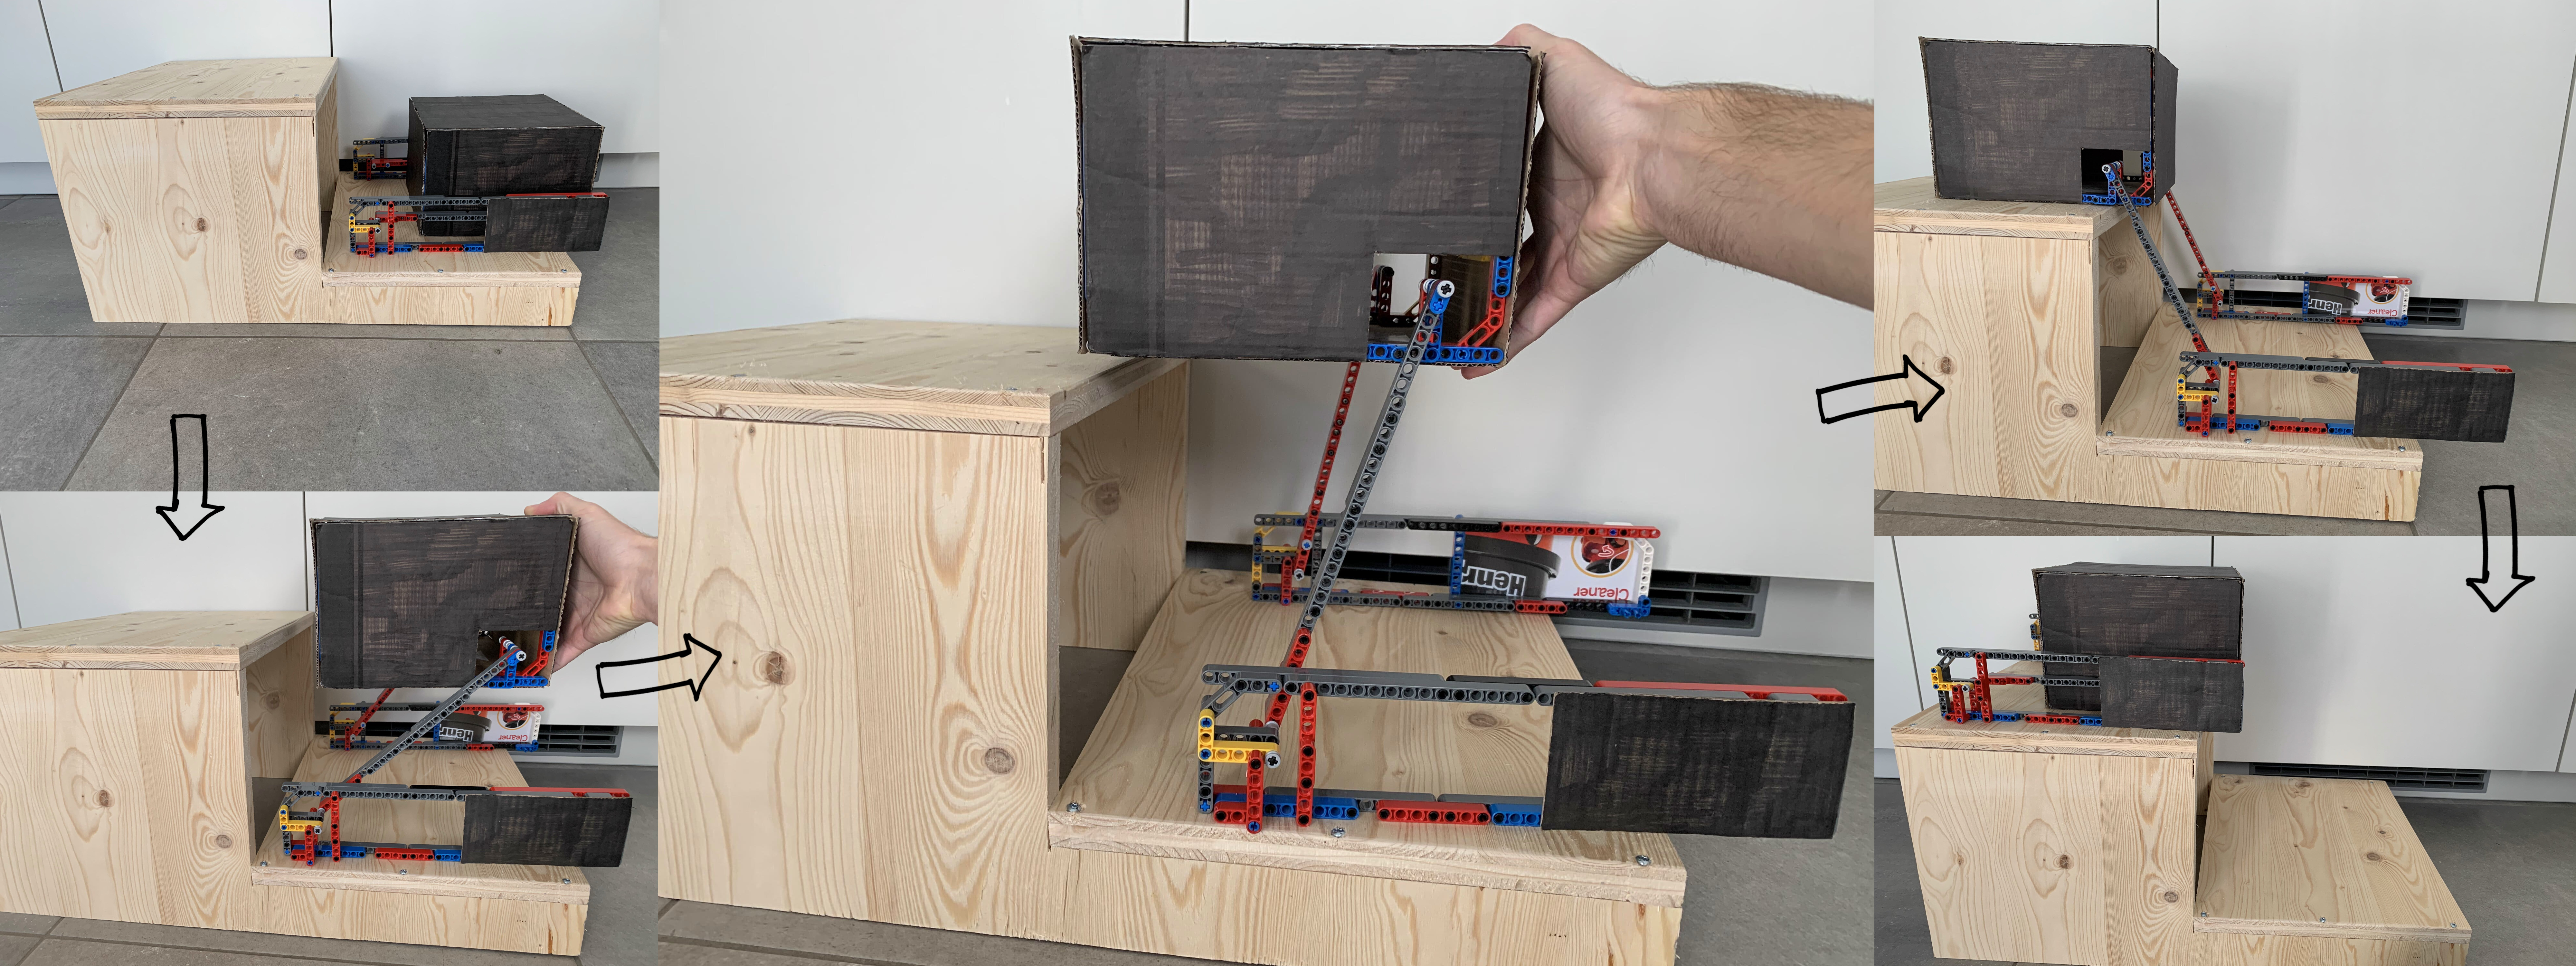
\includegraphics[width=0.8\textwidth]{img/stufenerklimmung.png}
  \centering
  \caption{Mockup für die Stufenerklimmung}
  \label{fig:mockup-stufenerklimmung}
\end{figure}
   
\newpage